\chapter{Elicited Monotonic Fairness} \label{ch:SoftMonoFair}

\newcommand{\xc}{c}

\section{Overview}

    The monotonicity constraint discussed in Chapter \ref{ch:MonoFair} ensures that the outcome has a monotonic relationship with individual attributes conditioned on the other attributes.  In practice, however, we often which to capture more complex definitions of ``better" attribute sets that consider multiple attributes at once.  For instance, consider the situation where two defendants are otherwise identical except that the first has committed ten more felonies and the second has committed one more misdemeanor; clearly, the first should be ranked as more likely to re-offend, but the two are incomparable according to these strict monotonicity rules.  In addition, such strict interpretation of monotonicity prevents comparison between individuals with non-identical covariates on non-monotonic axes, i.e. when the condition of otherwise identical attributes doesn't hold.  For example, if two defendants are 30 and 31 years old, they are incomparable.
    
    More complex concepts of monotonicity are difficult to capture a priori.  In this work, we explore the process of collecting and incorporating impartial arbiter information to ensure that individuals with commonly-accepted ``better" attributes will receiver favorable outcomes while maintaining predictive.  We do so by defining a loss function which depends only on the joint outcome of pairs so that arbiter comparisons can be combined with observed pairs of outcomes.  We operate in a conditional setting so that fairness and accuracy can be balanced post hoc as desired.    We also provide a means to incorporate group-level fairness to augment our individual-level protections.
    
    This section explores a methodology for eliciting such non-axial monotonicity based on surveying arbiters, which may or may not be fair in their judgments, and using those responses to regularize a classifier.  The input of the arbiters is motivated as preventing intuitive resentment. 

\section{Introduction}\label{sec:softmono_bg}
    
    We wish to extend the concept of \emph{non-protected attribute resentment} (Def. \ref{def:ScoreResentment}) to widen the comparisons which can be made when defining what is a ``better" $X_u$.
    
    At its core, the problem to be addressed is that an individual will have resentment toward others if the individual feels the others received better treatment despite not being as deserving.  Modeling each individual's views on relative treatment would be undesirable since we would like a rule which applies evenly to all individuals; we instead aim to learn a ranking function over individuals which can be used universally.  
    
    We propose to learn such a function by querying a set of arbiters by presenting pairs of non-protected attribute sets and asking for a judgment as to what the fair relative treatment of the pair would be. Once collected, these samples can be used to learn a \emph{preference function} over pairs of non-protected attributes that captures the arbiters' notion of monotonic fairness. Similarly, we can use the rankings implied by the data to learn a similar function that captures ground truth. We learn these two functions jointly, in a conditional setting. The idea is that learning the two functions jointly will act as a regularizer on the model learned on ground truth data, pulling it towards the arbiter's orderings, and (by changing the conditional variable at prediction time) we can extrapolate between a more accurate prediction of ground truth, and a more faithful representation of the arbiters' orderings.

    This is not the first work to incorporate the idea of utilizing arbiter queries in the area of fairness.  The original definition of individual fairness given by  \citet{dwork2012fairness} requires specifying a distance metric over attributes which can bound the difference in treatment, i.e. $D\left(f(X_i), f(X_j)\right) \le \kappa d(X_i, X_j)$. \citet{ilvento2019metric} and other recent works \citep{jung2019eliciting,lahoti2019operationalizing,wang2019empirical} approach the problem of operationalizing an individual fairness distance metric by polling arbiters on which pairs of individuals can be considered similar.  \citet{wang2019empirical} similarly collect actual survey data and evaluate a variety of models to interpret such data.  None of these approaches tackle the problem of dissimilar treatment, i.e. when an arbiter decides that two individuals should receive different predictions, especially the asymmetric case when arbiters indicate that one individual should receive a specifically more favorable or less favorable outcome than the other.
    
    Models which are designed to identify the relative values of pairs can be classified as preference learning models \citep{peters2018scalable}.  The problem of preference learning centers around the paradox that individuals with strong preferences are often unable to systematize those preferences in useful way  \citep{lichtenstein2006construction}.  A variety of methods have been proposed, including several Bayesian approaches \citep{peters2018scalable,guo2010gaussian} and neural network models  \citep{duman2019intelligent, khannoussi2019integrating} which propose methods of active preference elicitation.  This work does not elaborate on the process of preference elicitation, i.e. the optimization of queries for information gain, but instead focuses the incorporation of a preference function in resentment prevention and fairness.
    
    % We assume that the reader is familiar with the definitions and concepts in Sections \ref{sec:monofair_intro} and \ref{sec:monofair_background}.  

\section{Model}\label{sec:softmono_model}

    First, we define out variables closely to those in Chapter \ref{ch:MonoFair}.  We assume $(X, A) \in \mathcal{D} \subset \Omega$ with corresponding binary output $Y$.  Let $X^{obs}$, $Y^{obs}$, and $A^{obs}$ be the non-protected attributes, observed binary outcomes $\in \{0, 1\}$, and protected attributes for some set of $n$ individuals.  We assume an arbiter that we can query with pairs $X_i, X_j$ (or $(X_i, A_i), (X_j, A_j)$) and return an outcome $Z_{ij}^{arb} \in \{1, 2, 3, 4\}$, where the arbiters return 1 if it expects $f(X_i) > f(X_j)$, 2 if it expects $f(X_j) > f(X_i)$, 3 if it expects $f(X_i)$ and $f(X_j)$ to be similar, and 4 if it has no expectations as to the relative predictions.  We will generally refer to those $Z_{ij}^{arb} \in \{1, 2\}$ as \emph{dissimilar ratings} and those pairs $Z_{ij}^{arb} \in \{3\}$ as \emph{similar ratings}.
    
    We introduce an auxiliary variable $Z_{ij}^{obs}$ which captures relationships of $Y_i, Y_j$ in the observed data with parallel meaning:
    $$ Z_{ij}^{obs} = \left\{ \begin{array}{l c l}
        1 & \mbox{if} & Y_i^{obs} = 1 \mbox{~and~} Y_j^{obs} = 0 \\
        2 & \mbox{if} & Y_i^{obs} = 0 \mbox{~and~} Y_j^{obs} = 1 \\
        3 & \mbox{if} & Y_i^{obs} = Y_j^{obs}
    \end{array}\right. .$$
    
    The crux of this model is moving from optimizing for the direct prediction of outcomes encompassed by $Y$ to optimizing the relative outcomes encompassed by $Z$.  When we survey our fairness arbiters, we ask them to evaluate whether one individual is more likely ($Z = 1$), less likely ($Z = 2$), or similarly likely ($Z = 3$) than another specific individual to have $Y = 1$.
    
    We can then define a single loss function which incorporates both data sources:
    $$ \mathcal{L}_Z(Z, \hat{p}, \mathcal{Z}) = \sum\limits_{(i, j)} \left(\begin{array}{l} 
        \mathbf{1}_{Z_{ij} = 1} ~ \log\left( \hat{p}_i (1 - \hat{p}_j)  \right) ~ + \\
        \mathbf{1}_{Z_{ij} = 2} ~ \log\left( (1 - \hat{p}_i) \hat{p}_j  \right) ~ + \\
        \mathbf{1}_{Z_{ij} = 3} ~ \log\left(\hat{p}_i \hat{p}_j + (1 - \hat{p}_i)(1 - \hat{p}_j) \right)
        \end{array}\right), \label{eq:sm_pairwise_loss}$$
    letting $\mathcal{P}$ denote a set of pairs $(i, j)$ of size $|Z|$.
    
    In the above loss, the components for dissimilar outcomes can be reduced to the traditional log loss of the observed outcomes, i.e. if $Y_i^{obs} = 1$ and $Y_j^{arb}$ then 
        $ \log\left( \hat{p}_i (1 - \hat{p}_j)  \right) = \log\left( \hat{p}_i \right) + \log\left(1 - \hat{p}_j  \right)$ 
    is just the usual cross entropy loss.  For the case that $Z_{ij} = 3$, the loss component can be viewed as pushing $\hat{p}_i$ and  - $\hat{p}_j$ to take similar values; $\left(d \left(\hat{p}_i \hat{p}_j + (1 - \hat{p}_i)(1 - \hat{p}_j) \right)/d\hat{p_i}\right|_{\hat{p}_j} = 2\hat{p}_j - 1$, so that $\hat{p}_j$ is driven towards 0 if $\hat{p}_j < 1/2$ and towards 1 if $\hat{p}_j > 1/2$.  This is symmetric, so that if both estimates are pushed towards the same pole, with an unstable equilibrium if both are $1/2$.

    As mentioned above, we augment the neural network input with $\xc$, which acts as a conditional variable which is set to $\xc = 0$ when we wish to predict according to the observed data without concern for agreement with intuitive resentment, and which is set $\xc = 1$ when we wish to predict according to our arbiter data (and possibly a group fairness constraint) without concern for predictive accuracy according to the observed data.  This design allows us to a tune a prediction continuously between being based entirely on real data without concern for agreeing with intuitive resentment and being based entirely on the arbiter data at the expense of predictive accuracy.
    
    We can further add other losses to the prediction task when $\xc = 1$, e.g. a differentiable loss on a variant of group fairness like equality of outcome, odds, or opportunity.  We assess this only on the predictions when $\xc = 1$ since that conditional setting corresponds to the ``fair" setting; this effect of this loss can then also be balanced by setting $\xc \in (0, 1)$.

\section{Experiments}\label{sec:softmono_experiments}

    We demonstrate the use of the above pairwise loss on two datasets.  First, in Section \ref{subsec:sm_synthetic} we consider a synthetic experiment without protected attributes where the true probability $\Pr(Y_i = 1 | X_i)$ is known and we attempt to recover that probability using a simple feedforward neural network, as described in Sections \ref{sec:intro_nns} and \ref{sec:monofair_experiments}, trained to minimize \ref{eq:sm_pairwise_loss}.  
    
    Second, in Section \ref{subsec:sm_compas} we consider the COMPAS dataset, and utilize human survey responses and attempt to learn a network with a conditional prediction structure which allows for post-hoc compromise between fairness loss and prediction accuracy.

    \subsection{Synthetic - Proof of balancing objectives}\label{subsec:sm_synthetic}
    
        We begin with a synthetic experiment where the ground truth is known.  We have an individual set of attributes $X_i \sim N(0, 1)^2$, and two weight vectors,  $\beta_{obs} = [0.9, 1.1]$ and $\beta_{arb} = [1.1, 0.9]$, which describe the relationship between $X$ and, respectively,  $Z_{ij}^{obs}$ (via $Y_{i}^{obs}$) and $Z_{ij}^{arb}$.  We set $P_i^{obs} = 1 / (1 + \exp\{-X_i \beta^{obs} - 1\})$, sample $Y_i \sim \mbox{Bernoulli}(P_i^{obs})$, and set $Z_{ij}^{obs}$ as defined as above.  We set $Z_{ij}^{arb}$ according to:
            $$ Z_{ij}^{arb} = \left\{ \begin{array}{lll}
                    1 & \mbox{if} & X_{i}\beta^{arb} > X_{j}\beta^{arb} + 0.25\\
                    2 & \mbox{if} & X_{j}\beta^{arb} > X_{i}\beta^{arb} + 0.25 \\
                    3 & \mbox{if} & | X_{i}\beta^{arb} - X_{j}\beta^{arb} | < 0.25
                \end{array} \right. .$$
        We sample 1,000 training examples of $Z_{ij}^{obs}$ and 200 examples of $Z_{ij}^{arb}$, and evaluate losses on the same number of identically distributed held out samples.  We trained using a small neural network of three hidden layers of width three and a $\tanh$ activation function. We optimize for a compound loss,
            $$\mathcal{L} = \underbrace{\mathcal{L}_Z\left(Z_{ij}^{obs}, \hat{p}_i = f(X_i, \xc = 0), \mathcal{O} \right)}_{\mathcal{L}_Z^{obs}}
                          + \underbrace{\mathcal{L}_Z\left(Z_{ij}^{arb}, \hat{p}_i = f(X_i, \xc = 1), \mathcal{A} \right)}_{\mathcal{L}_Z^{arb}} 
                          + g(\theta)$$
        where $\mathcal{O}$ is the set (or a subset) of pairs of observations, $\mathcal{A}$ is the set of arbiter-assessed pairs, and $g(\theta)$ is a regularization term on the parameters of the network.  We arbitrarily set $g(\theta) = 0.01 * \left(||\theta||_1 + ||\theta||_2^2\right)$ to provide weak regularization of the network.
        
        First, we wish to establish that the pairwise loss defined above can be used to estimate the probability function underlying probability function when $\xc = 0$ i.e. when attempting to predict based purely on the observed outcomes via the $Z_{ij}$ pairs.  In Figure \ref{fig:sm_synthetic_p_fit}, we show experimentally that $\hat{P}_i$ is accurate to within the limit of sampling error and (intentional) model misspecification.
        
        \begin{figure}
            \centering
            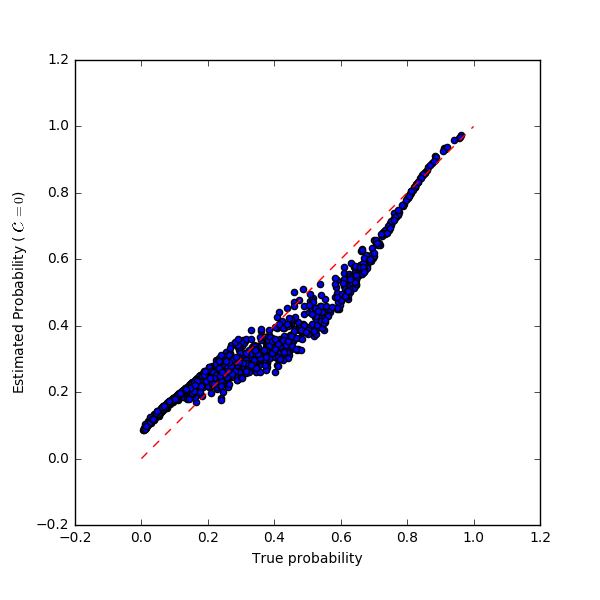
\includegraphics{fig_softmono/synthetic_p_fit.png}
            \caption{The model estimated probability of $\Pr(Y_i = 1 | X_i, \xc = 0)$ versus the ground truth probabilities, with 1:1 line.}
            \label{fig:sm_synthetic_p_fit}
        \end{figure}
        
        Second, we wish to assess whether the model is able to interpolate via $\xc$ between it's dual goals of predicting $\hat{Y}_i$ while adhering to the surveyed $Z_{ij}^{arb}$ pairs.  The trend of $Z_{ij}^{arb}$ is exactly as expected; lowest when $\xc = 0$ and gradually increasing to a maximum when $\xc = 1$.  The behavior of $Z_{ij}^{arb}$ is less intuitive; it is highest when $\xc = 0$, but many random fits have an local minimum loss with $\xc < 1$.  This is explained by the relatively small sample ($n^{arb} = 200$) leading to overfitting even in this modest network, and by $\mathcal{L}_Z^{obs}$ providing regularization which improves out-of-sample performance.  We also, when examining the joint loss values available, that the models fits form appropriate trade off functions for performance, with reduction of one loss coming at the cost of increase of the other. 
        
        \begin{figure}
            \centering
            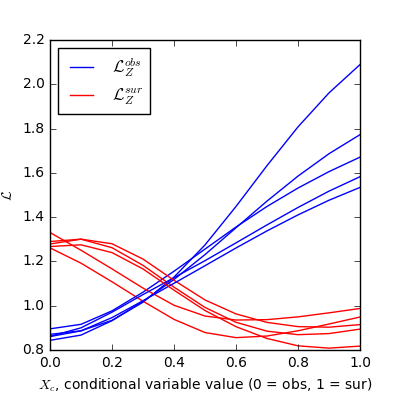
\includegraphics[width=0.45\textwidth]{fig_softmono/synthetic_loss.png}
            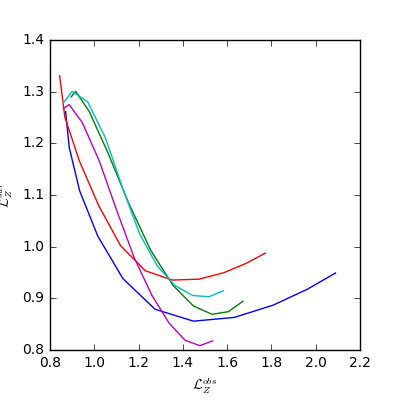
\includegraphics[width=0.45\textwidth]{fig_softmono/synthetic_loss_tradeoff.png}
            \caption{
                Model losses as a function of conditional variable ($\xc$) setting over 5 experiments with random initializations.  Left: losses as a function of $\xc$, with $\mathcal{L}_Z^{obs}$ in blue and $\mathcal{L}_Z^{arb}$ in red.  Right: parametric plot of $\mathcal{L}_Z^{arb}$ as a function of $\mathcal{L}_Z^{obs}$.
            }
            \label{fig:sm_synthetic_losses}
        \end{figure}
        
    \subsection{COMPAS}\label{subsec:sm_compas}
    
        We augment the COMPAS dataset described in Section \ref{sec:monofair_experiments} in two ways: we add a feature for whether the current charge is violent, and we collect survey data to on random pairs and the possible ordering of their outcomes.
        
        First, in adding the feature for violence of the current charge, we used the classification system described by ProPublica \citep{larson2016we} and based on the US Department of Justice's definition of a violent crime: ``murder and nonnegligent manslaughter, forcible rape, robbery, and aggravated assault."  With this feature added, the non-protected attributes are age, (adult) priors count, juvenile prior felony count, juvenile prior misdemeanor count, juvenile prior other counts, arrest charge degree (felony or misdemeanor), and whether the arrest charge is violent.  The protected attributes are race, classified as Caucasian, African American, or Other (comprising what the dataset labels as Other, Hispanic, Native American, and Asian), and Sex, classified as Male or Female.
        
        The second augmentation was made by survey.  Five volunteers were each presented 100 independent random pairings of non-protected attributes, i.e. excluding the protected attributes of race and sex.  For each pairing, the two individuals were labeled ``Individual A" and ``Individual B", and the arbiter asked to provide one of four ratings:
        \begin{itemize}
            \item ``A is at least as likely to (re)offend" ($Z = 1$)
            \item ``B is at least as likely to (re)offend" ($Z = 2$)
            \item ``A and B are similarly likely to (re)offend" ($Z = 3$)
            \item ``No preference / any of the others are fair"
        \end{itemize}
        % The full survey instructions are presented in the appendix. % I might add this back in time permitting.  
        Seventeen responses indicating no preference were discarded, leaving 298 dissimilar responses ($Z \in \{1, 2\}$) and 185 similar responses ($Z = 3$).

        We make no claim that the arbiters we surveyed have any qualification as unbiased judges; in the current setting where we do not provide protected attributes, the role of these arbiters is not to provide protected attribute-aware judgments.  Instead, they are intended to provide feedback on what conditions they would find unfair via the individuals who should be more (or less) likely to get bail than others.  This doesn't require expert knowledge because resentment occurs at an individual, non-expert level.

        For group fairness loss, we chose to evaluate equality of odds, which requires that the prediction is independent of the protected attributes conditioned on the true outcome, i.e.
            $$ \Pr(\hat{Y} = 1 | A = a, Y = y) = \Pr(\hat{Y} = 1 | A = a', Y = y) \forall a, a', y .$$
        We express this is a differentiable loss as 
            $$ \mathcal{L}_F = \sum\limits_{y} \sum\limits_{a} \left( \bar{\hat{y}}_{ay} - \bar{\hat{y}}_{\cdot y} \right)^2 $$
        where $\bar{\hat{y}}_{ay} = \sum_{i: A_i = a, Y_i = y}(\hat{Y}_i) / n_{ay}$, i.e. the average prediction individuals of each protected attribute set and true outcome, and $\bar{\hat{y}}_{\cdot y} = \sum_{i: Y_i = y}(\hat{Y}_i) / n_{\cdot y}$, i.e. the average prediction for all individuals of that true outcome.  Note that, as described above, we will always assess $\mathcal{L}_F$ using estimates $\hat{y}$ conditioned on $\xc = 1$, i.e. in the conditional setting where we care about fairness, both individual and group. 
        
        We then set our training loss, using the notation from the synthetic experiment above, as
            $$\begin{array}{l l}
                \mathcal{L} = & 
                    \underbrace{\mathcal{L}_Z\left(Z_{ij}^{obs}, f(X_i, \xc = 0)\right)}_{\mathcal{L}_Z^{obs}}
                    + \underbrace{\mathcal{L}_Z\left(Z_{ij}^{arb}, f(X_i, \xc = 1)\right)}_{\mathcal{L}_Z^{arb}} 
            \\ &    + \lambda_F \underbrace{\sum\limits_{y \in \{0, 1\}} \sum\limits_{a \in \mathcal{A}} \left( \bar{\hat{y}}_{ay} - \bar{\hat{y}}_{\cdot y} | \xc = 1 \right)^2}_{\mathcal{L}_F} 
                    + g(\theta)
            \end{array} $$
            % $$\mathcal{L} = \mathcal{L}_Z^{obs}
            %               + \mathcal{L}_Z^{arb}
            %               + \lambda_F \mathcal{L}_F
            %               + g(\theta).$$
        where $\lambda_F$ is a parameter to weight $\mathcal{L}_F$ relative to $\mathcal{L}_Z^{arb}$.
        
        Due to the increased data set size and complexity, we use a larger network in this problem with 4 hidden layers each of size 10.  As long as we assume that axial monotonicity as discussed in Chapter \ref{ch:MonoFair} applies, we can train the present network using either a traditional feedforward neural network or the monotonic neural previously discussed; we present results from only the former to limit uncontrolled factors.
        
        \begin{figure}
            \centering
            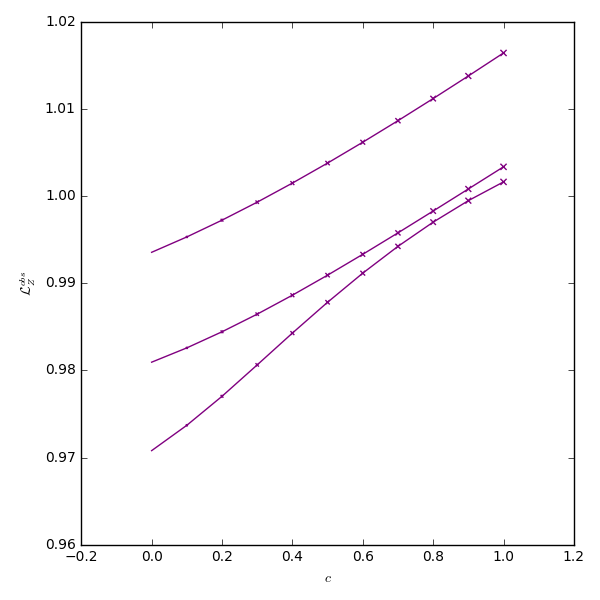
\includegraphics[width=.45\textwidth]{fig_softmono/compas_lzo_c.png}
            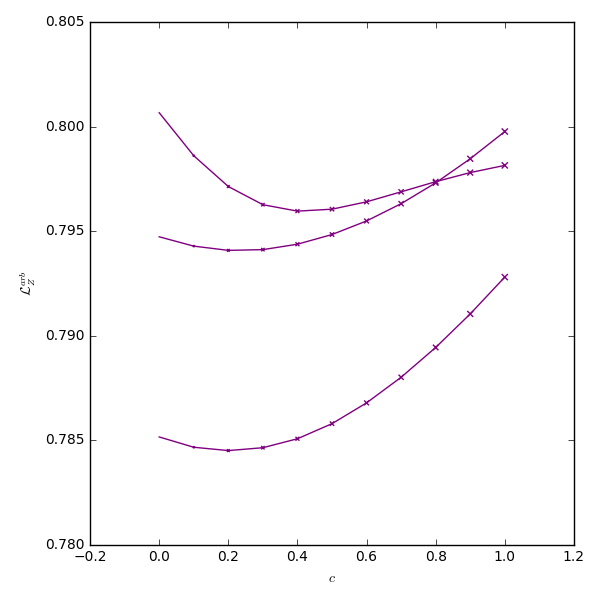
\includegraphics[width=.45\textwidth]{fig_softmono/compas_lzs_c.png}
            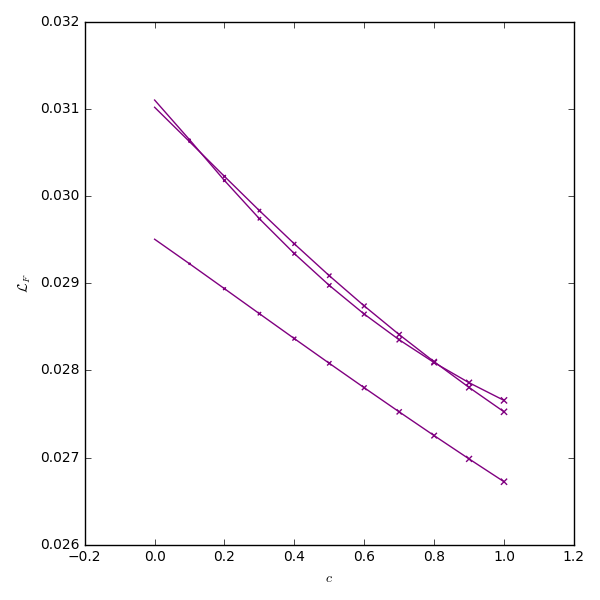
\includegraphics[width=.45\textwidth]{fig_softmono/compas_lf_c.png}
            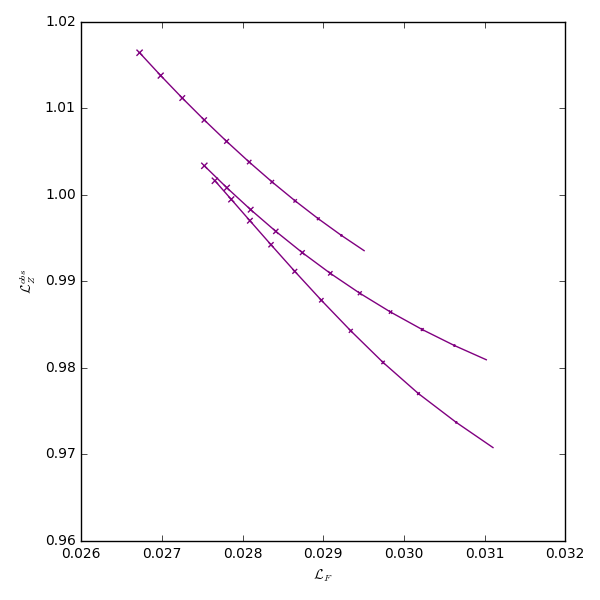
\includegraphics[width=.45\textwidth]{fig_softmono/compas_lzo_lf.png}
            \caption{Clockwise from top left: Pairwise loss on observed data $\mathcal{L}_Z^{obs}$  as a function of $c$, pairwise loss on arbiter data $\mathcal{L}_Z^{arb}$ as a function of $c$, group fairness loss $\mathcal{L}_F$ as a function of $c$, and $\mathcal{L}_Z^{obs}$ as a function of group fairness loss $\mathcal{L}_F$.  Lines represent three random training runs with $\lambda_f = 0.001$.  Marker size is proportionate to $c$.}
            \label{fig:sm_compas_tradeoffs}
        \end{figure}
        
        In Figure \ref{fig:sm_compas_tradeoffs}, we examine experimental results.  Similar to our synthetic experiment, the pairwise loss on observed data $\mathcal{L}_Z^{obs}$ is lowest when $c = 0$ and increases steadily toward $c = 1$.  The fairness loss $\mathcal{L}_F$ has a similar but opposite trend, and has an expected tradeoff curve with $\mathcal{L}_Z^{obs}$
        
        An interesting anomaly, however, is the trend for the pairwise loss on arbiter data $\mathcal{L}_Z^{arb}$ (top right), which is highest at $c = 1$ when we would naively expect it to be lowest.  Counterintuitively, this is explained by the fact that the arbiter ratings, which are assumed to be fair w.r.t.~resentment but are in fact severely biased w.r.t group fairness.  For instance, despite being unaware of race, arbiters' views on relative treatment led them to rate the non-protected attributes of African-Americans as more likely to re-offend than those of Caucasians on average; in the 105 ratings where they gave a dissimilar rating for an African-American and Caucasian pairing, they rated the African American defendant's non-protected attributes as more likely to re-offend 68 times (65\%). The result of this contradiction in arbiter-based individual fairness and group fairness is predictable: one of them dominates when $c=1$, and in this case it is group fairness, likely due to loss scaling.  
        
        Another factor causing $\mathcal{L}_Z^{arb}$ to be lower towards $c=0$: the arbiters are actually fairly accurate.  Of the 164 dissimilar ratings given, 128 ratings (78\%) were directionally correct, which is comparable accuracy to a roughly three point difference on the COMPAS decile score system, despite COMPAS having access to additional attributes (both protected and other) that we didn't reveal to the arbiters. This relatively high accuracy of arbiter ratings allows them to act as additional information for training the structure of the classifer, improving the accuracy when $c=0$ (and $c$ \emph{near} 0), even if no loss considers the accuracy of arbiter ratings when $c = 0$. 
        
    \section{Discussion}\label{sec:sm_discussion}
    
        The ability to incorporate preference learning into fairness models allows us to prevent individual resentment without a priori knowledge of what treatments would cause resentment.  Such a priori knowledge is often hard to come by, requiring expert knowledge and a well structured problem.  When such knowledge is available, it can still be difficult to systematize that a prior knowledge into a method for exact comparisons.  We have shown a method for eliciting data informative of that a priori knowledge from arbiters via surveys, incorporating that data into a statistical model of preferences, and providing post hoc-tunable prediction which respects that arbiter input and, hopefully, prevents indvidiuals treated by the system from experiencing indvidual resentment. 
        
        The current work opens future research questions as well.  While there are many methods available for preference function learning, they  have not been widely integrated into the fairness literature.  Integration of preference learning, and especially direct inference of the arbiter preference resulting in a well defined preference function, would open opportunities for an improved system with better guarantees. Although we have a loss function which can direct balance the observed and arbiter-provided data, we have not shown an easily-tuned system for incorporating more commonly used group fairness metrics.  In addition, the current work is focused on neural networks and controlling violations of arbiter-provided ratings by loss penalization; it would be desirable to provide the hard guarantees non-resentment that is available for axial monotonicity.